
Regardless the manner how the quench velocity is calculated, Python script will always understand the quench length as if it was a continuous function of time. Therefore, it is expected that the calculated quench position ~$L$ in a given time in Python script will differ from the available positions of a discrete meshed ANSYS geometry. 

The searching node algorithm is presented in Fig. \ref{fig:node_search_algo}. It searches the node $N_\text{search}$ whose geometric position is below the assumed error,~$\epsilon$ compared to the quench length $L$ calculated on the Python side. At each time step the algorithm checks whether $N_\text{search}$ is within the space $N$ and ${N+x}$ when jump search is considered. In case of a dense mesh, the step control doubles if the right zone ${[N+(a-1)x, N+ax]}$ is not found after 5 iterations. When the node space ${[N+(a-1)x, N+ax]}$ contains the searched node, it uses the binary search to find the node fulfilling the condition ${\mid L(N_\text{search}) - L \mid \geq \epsilon}$. 

\begin{figure}[H]
\centering
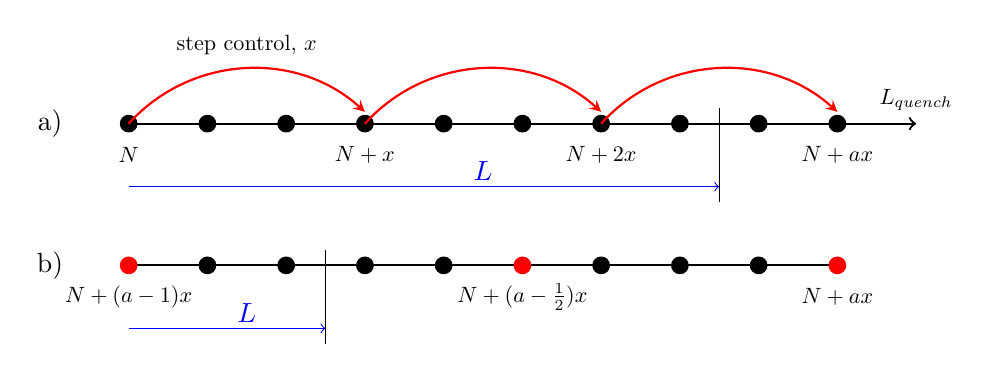
\begin{tikzpicture}[scale = 1]
\draw[thick,->] (0,1) -- (10,1);
\foreach \t in {0,1,...,9}
\filldraw[black] ({\t},1) circle (3pt);
\foreach \t in {1,4,7}
\draw [thick, -stealth, bend angle=45, bend left, color = red]  ({\t-1},1) to (\t+2,1.15);
\node[scale = 0.8] at (1.5, 2) {step control, $x$};
\node[scale = 0.8] at (0, 0.6) {$N$};
\node[scale = 0.8] at (3, 0.6) {$N+x$};
\node[scale = 0.8] at (6, 0.6) {$N+2x$};
\node[scale = 0.8] at (9, 0.6) {$N+ax$};
\node[scale = 0.8] at (10, 1.3) {$L_{quench}$};
\draw[thin, blue, ->] (0,0.2) -- (7.5,0.2);
\draw[thin, black] (7.5,0) -- (7.5,1.2);
\node[scale = 1, blue] at (4.5, 0.4) {$L$};
\node at (-1, 1) {a)};

\draw[thick] (0,-0.8) -- (9,-0.8);
\foreach \t in {1,2,3,4,6,7,8}
\filldraw[black] ({\t},-0.8) circle (3pt);
\foreach \t in {0,5,9}
\filldraw[red] ({\t},-0.8) circle (3pt);
\node[scale = 0.8] at (0, -1.2) {$N+(a-1)x$};
\node[scale = 0.8] at (5, -1.2) {$N+(a-\frac{1}{2})x$};
\node[scale = 0.8] at (9, -1.2) {$N+ax$};
\draw[thin, black] (2.5,-1.8) -- (2.5,-0.6);
\draw[thin, blue, ->] (0,-1.6) -- (2.5,-1.6);
\node[scale = 1, blue] at (1.5, -1.4) {$L$};
\node at (-1, -0.8) {b)};
\end{tikzpicture}
\caption{ a) Jump search; b) Bi-section search}
\label{fig:node_search_algo}
\end{figure}

Provided that searching starts at node $N$, quench length calculated in Python is $L$, searching error is $\epsilon$, step control equals $x$, number of step controls applied equals $a$, the problem is solved as described in Algorithm \ref{alg:node_searching}.

\begin{algorithm}
    \caption{Node Searching}
    \label{alg:node_searching}
    \begin{algorithmic}[1]
    \STATE \textbf{while} $L(N) < L$ \textbf{do}
    \STATE \hspace{0.5cm} increase N by step control x
    \STATE \hspace{0.5cm} \textbf{if} number of iterations over x is multiplication of 5 \textbf{do}
    \STATE \hspace{1.0cm} double step control $x$
    \STATE \textbf{while} $\mid L(\frac{2N+(2a-1)x}{2}) - L \mid \geq \epsilon$ \textbf{do}
    \STATE \hspace{0.5cm} \textbf{if} $L(\frac{2N+(2a-1)x}{2}) > L$ \textbf{do}
    \STATE \hspace{1.0cm} continue search in domain $D \in (N+(a-1)x ; \frac{2N+(2a-1)x}{2})$
    \STATE \hspace{0.5cm} \textbf{elseif} $L(\frac{2N+(2a-1)x}{2}) < L$ \textbf{do}
    \STATE \hspace{1.0cm} continue search in domain $D \in (\frac{2N+(2a-1)x}{2} ; N+ax)$
    \end{algorithmic}
\end{algorithm}

The algorithm also works if the mesh is too coarse or if $\epsilon$ is too small to find the right node with binary search. In such a case, the closest node to analytic length is chosen.